\documentclass[DIN, pagenumber=false, fontsize=11pt, parskip=half]{scrartcl}

\usepackage{amsmath}
\usepackage{amsfonts}
\usepackage{amssymb}
\usepackage{enumitem}
\usepackage[utf8]{inputenc} 
\usepackage[ngerman]{babel} 
\usepackage[T1]{fontenc} 
\usepackage{pgfplots}
\usepackage{xcolor}
\usepackage{listings}
\usepackage{float}
\usepackage{graphicx}

\definecolor{mygreen}{RGB}{28,172,0} % color values Red, Green, Blue
\definecolor{mylilas}{RGB}{170,55,241}

\lstset{language=Matlab,%
    %basicstyle=\color{red},
    breaklines=true,%
    morekeywords={matlab2tikz},
    keywordstyle=\color{blue},%
    morekeywords=[2]{1}, keywordstyle=[2]{\color{black}},
    identifierstyle=\color{black},%
    stringstyle=\color{mylilas},
    commentstyle=\color{mygreen},%
    showstringspaces=false,%without this there will be a symbol in the places where there is a space
    numbers=left,%
    numberstyle={\tiny \color{black}},% size of the numbers
    numbersep=9pt, % this defines how far the numbers are from the text
    emph=[1]{for,end,break},emphstyle=[1]\color{red}, %some words to emphasise
    %emph=[2]{word1,word2}, emphstyle=[2]{style},    
}

\title{Computer Vision I}
\author{Tim Luchterhand, Paul Nykiel (Group 17)}

\begin{document}
    \maketitle
    \section{Histogram Calculation}
    \begin{enumerate}
        \item Matlab-Funktion: \lstinputlisting{myHistogram.m}
        \item Generate the plots: \lstinputlisting{sh01ex01.m}
        \item  $ $
            \begin{figure}[H]
                \centering
                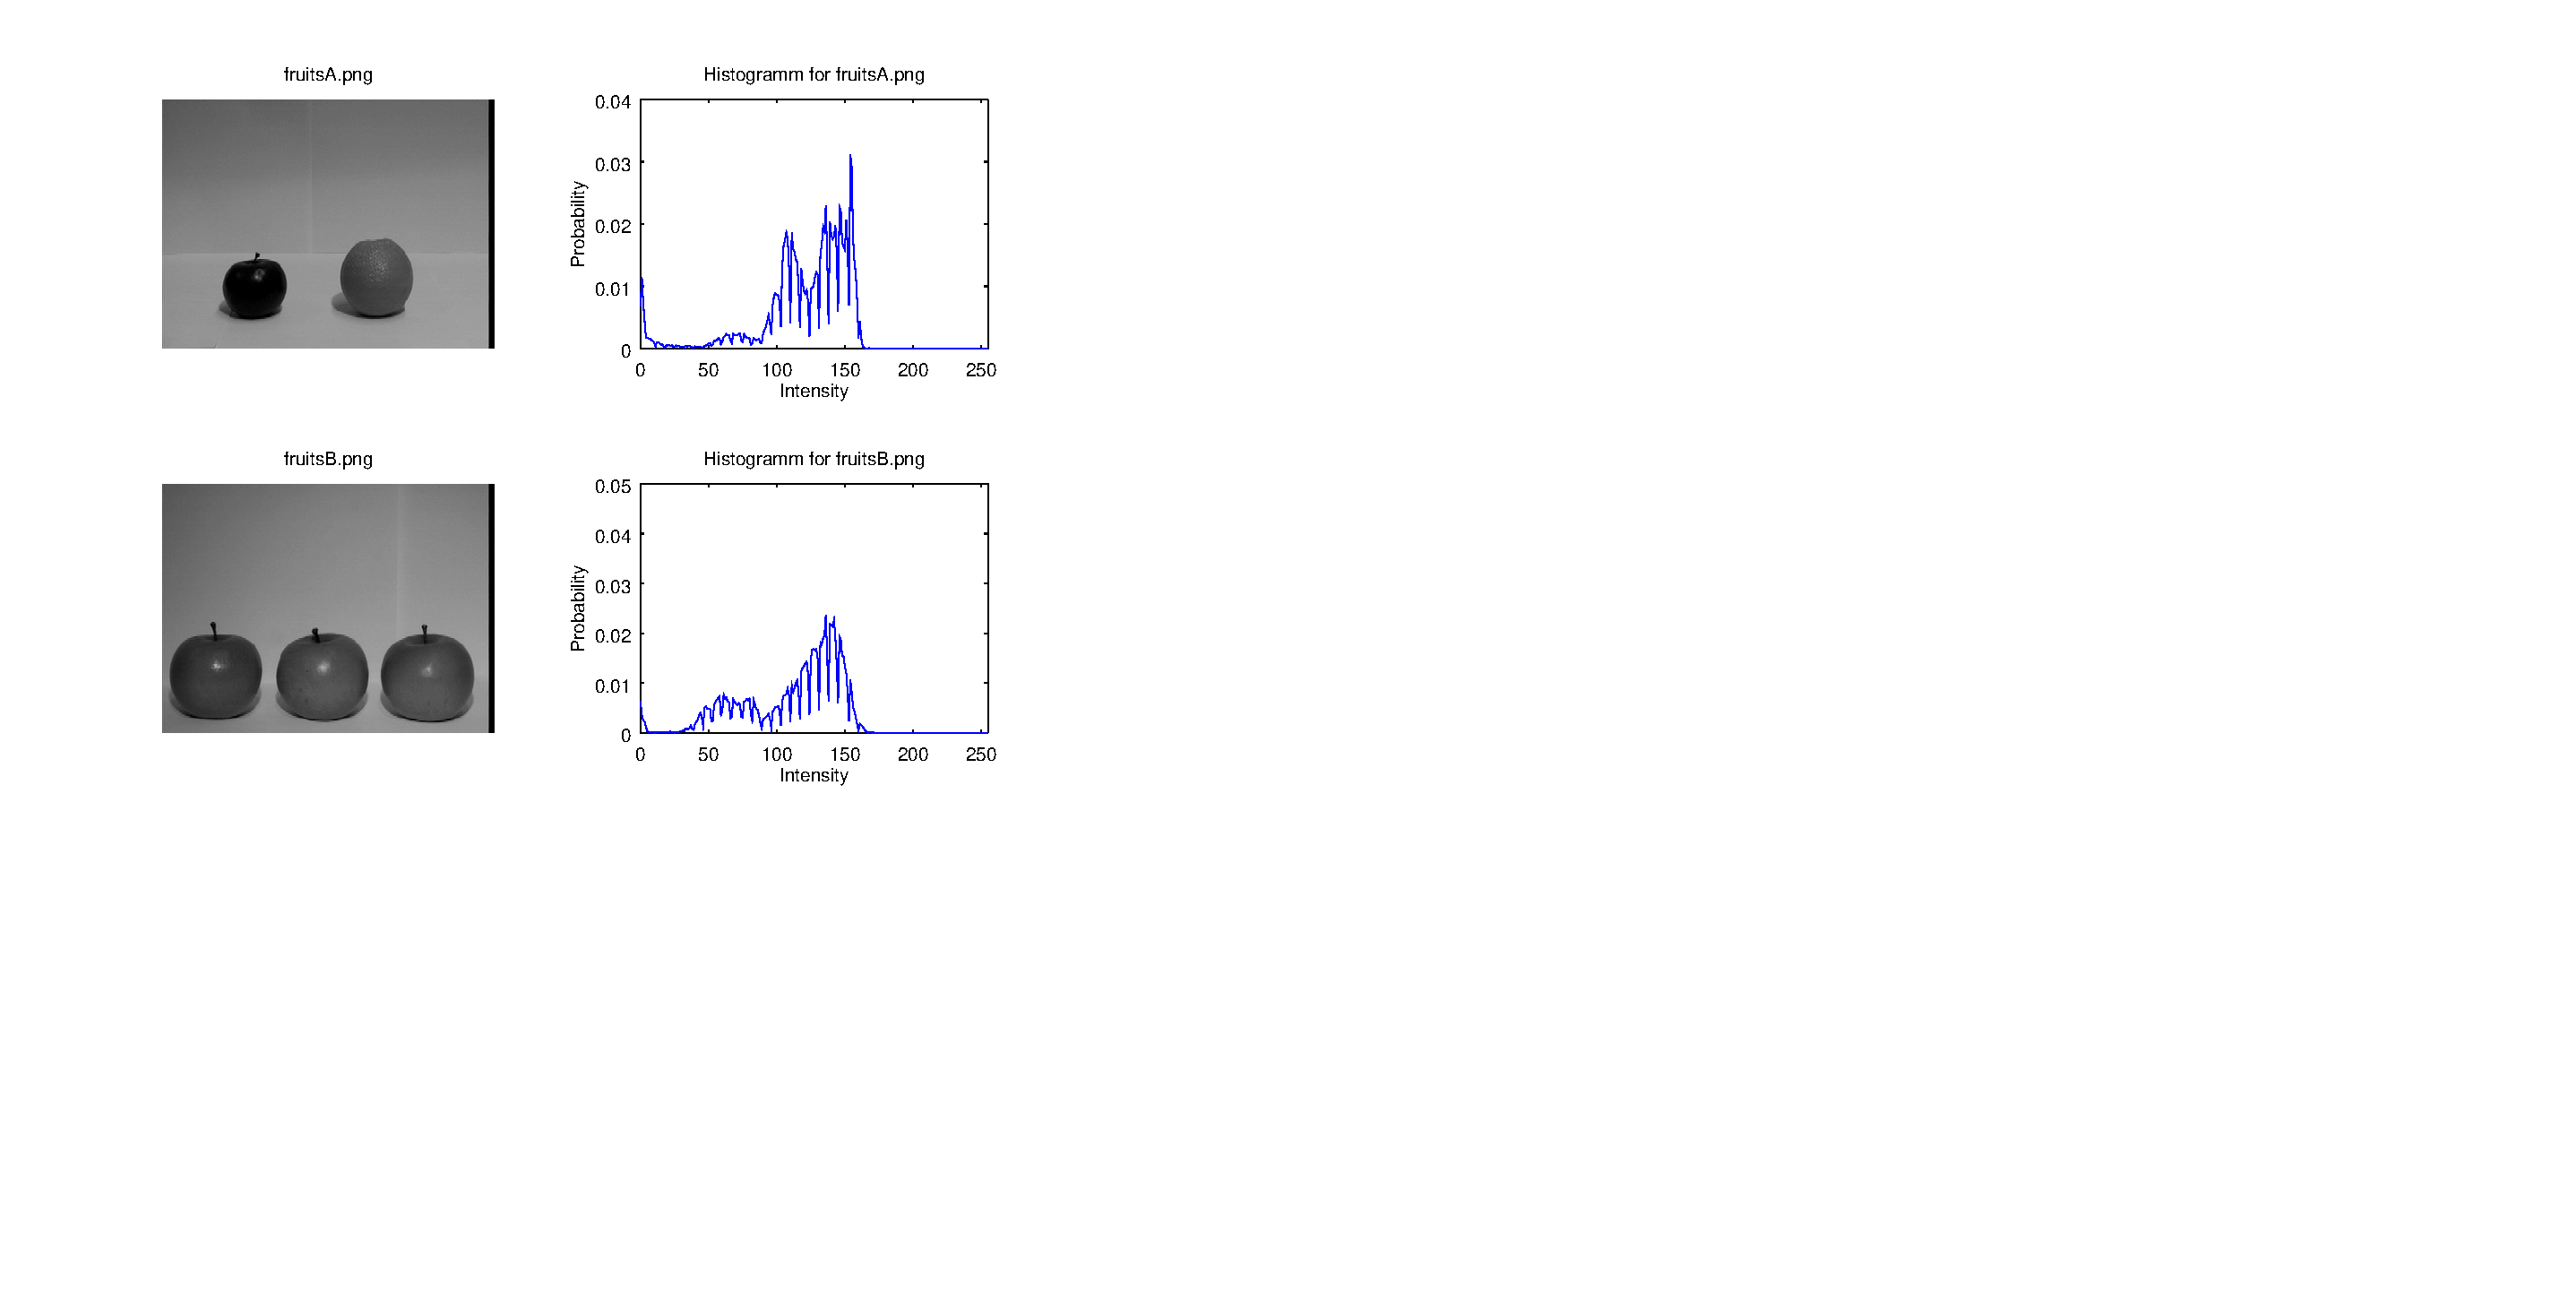
\includegraphics[trim = {0 9cm 27cm 0}, clip,width=\textwidth]{Histograms}
                \caption{Plot of the histograms}
            \end{figure} 
        \item $ $
            \begin{figure}[H]
                \centering
                \begin{tikzpicture}
                    \node[anchor=south west,inner sep=0] at (0,0) {
                        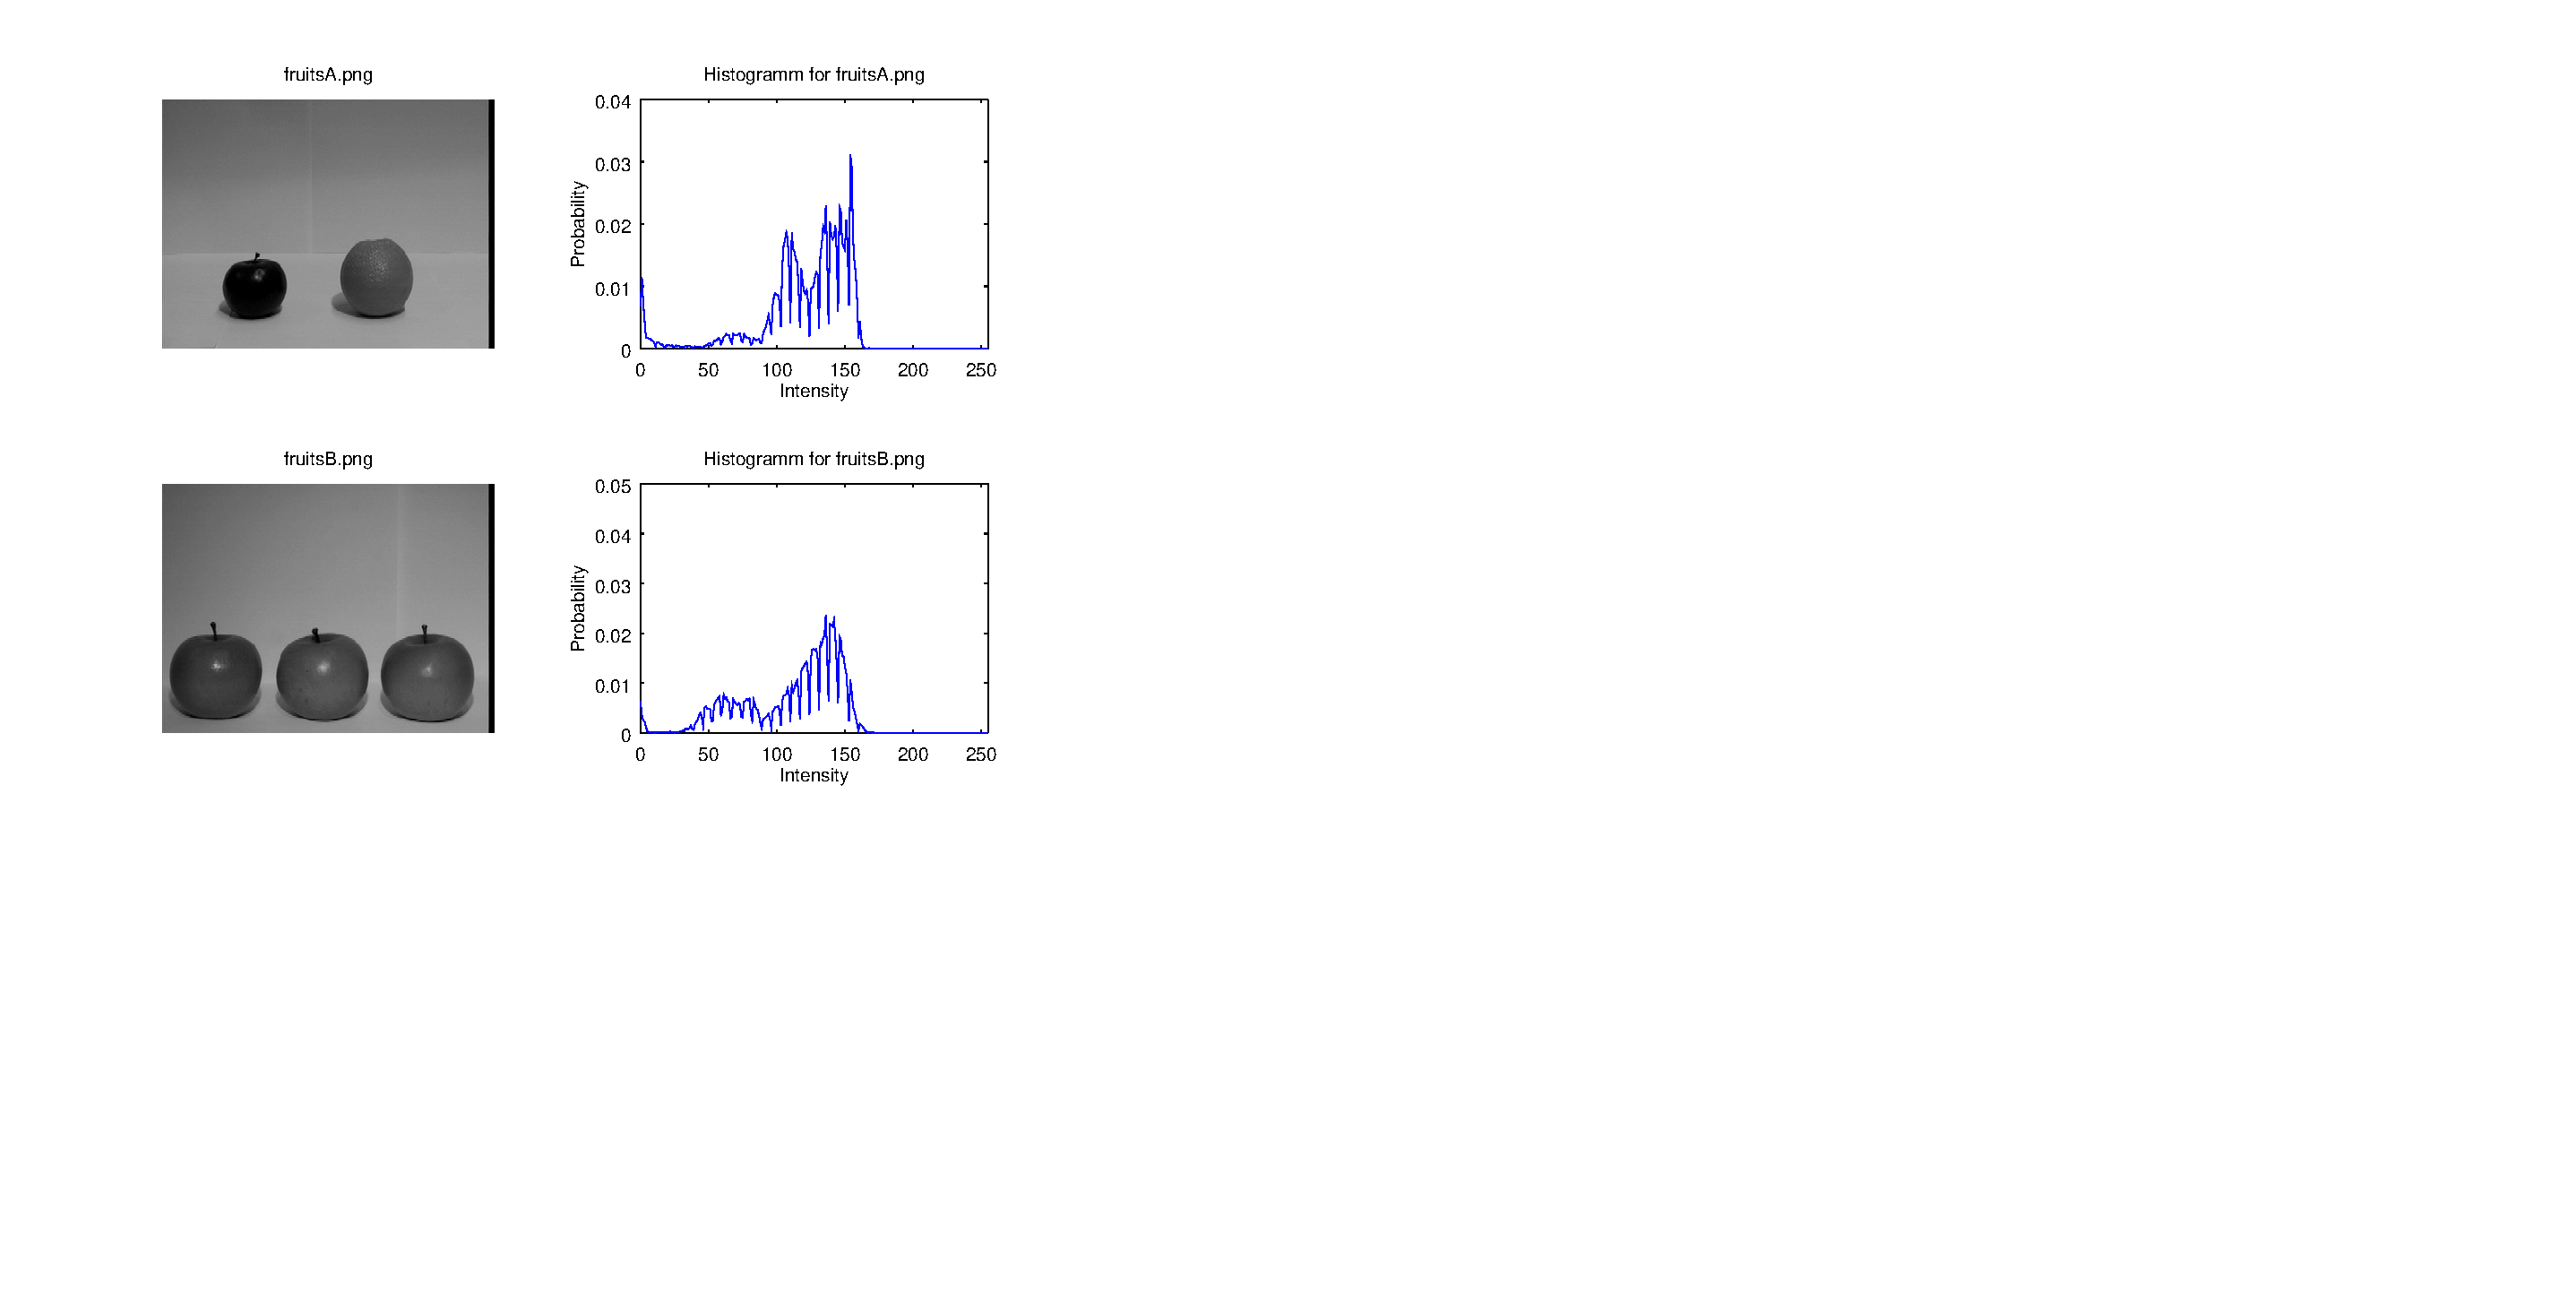
\includegraphics[trim = {0 9cm 27cm 0}, clip,width=\textwidth]{Histograms}
                    };
                    \node at (8.6,8) {\scriptsize Apple};
                    \node at (9.5,8) {\scriptsize Orange};
                    \node at (10.6,9) {\scriptsize Background};

                    \node at (9.4,3) {\scriptsize Apples};
                    \node at (10.6,4) {\scriptsize Background};
                \end{tikzpicture}
                \caption{Plot of the histograms}
            \end{figure} 
        \item $ $
            \begin{figure}[H]
                \centering
                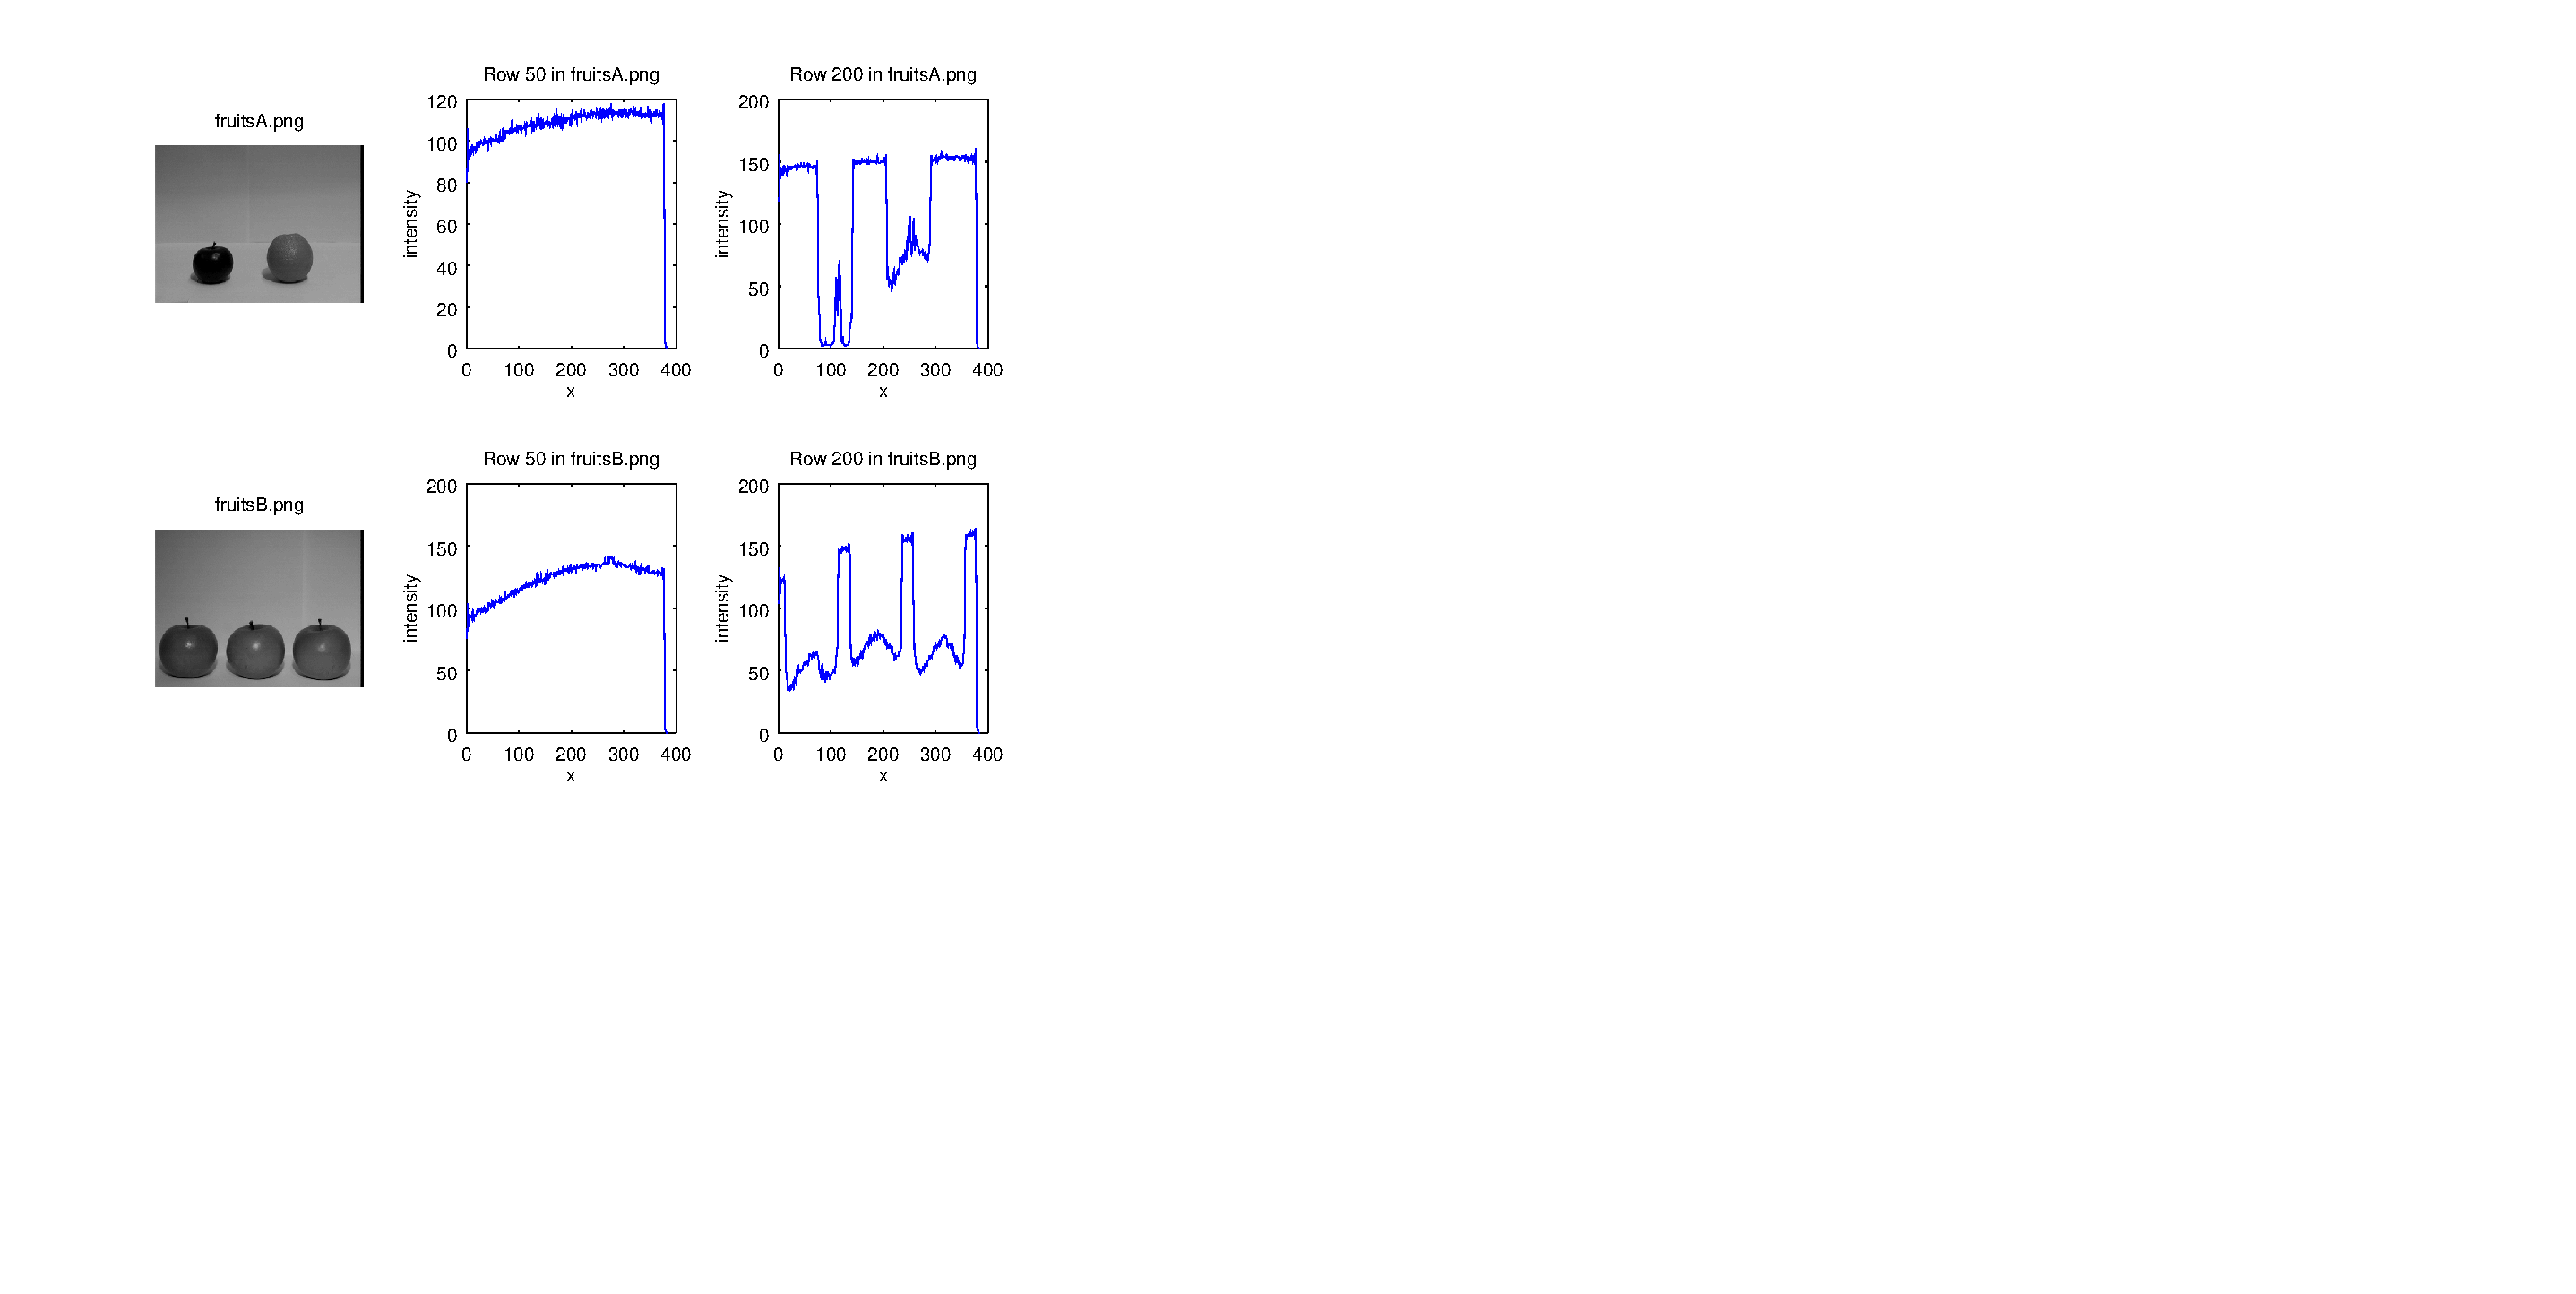
\includegraphics[trim = {0 9cm 27cm 0}, clip,width=\textwidth]{Rows}
                \caption{Plot of the rows}
            \end{figure} 
    \end{enumerate}
    \section{Local weighting}
    \begin{enumerate}
        \item 
            \begin{equation*}
                \begin{pmatrix}
                    \cdot & \cdot & \cdot & \cdot \\
                    1 \cdot 1 + 1 \cdot 1 & 1 \cdot 1 & -1 \cdot 1 + -1 \cdot 1 + 1 \cdot 1  & \cdot \\
                    \cdot & \cdot & \cdot & \cdot \\
                    \cdot & \cdot & \cdot & \cdot
                \end{pmatrix} =
                \begin{pmatrix}
                    \cdot & \cdot & \cdot & \cdot \\
                    2 & 1 & -1 & \cdot \\
                    \cdot & \cdot & \cdot & \cdot \\
                    \cdot & \cdot & \cdot & \cdot
                \end{pmatrix}
            \end{equation*}
        \item TODO
        \item $ $ \lstinputlisting{sh01ex02.m}
            \begin{figure}[H]
                \centering
                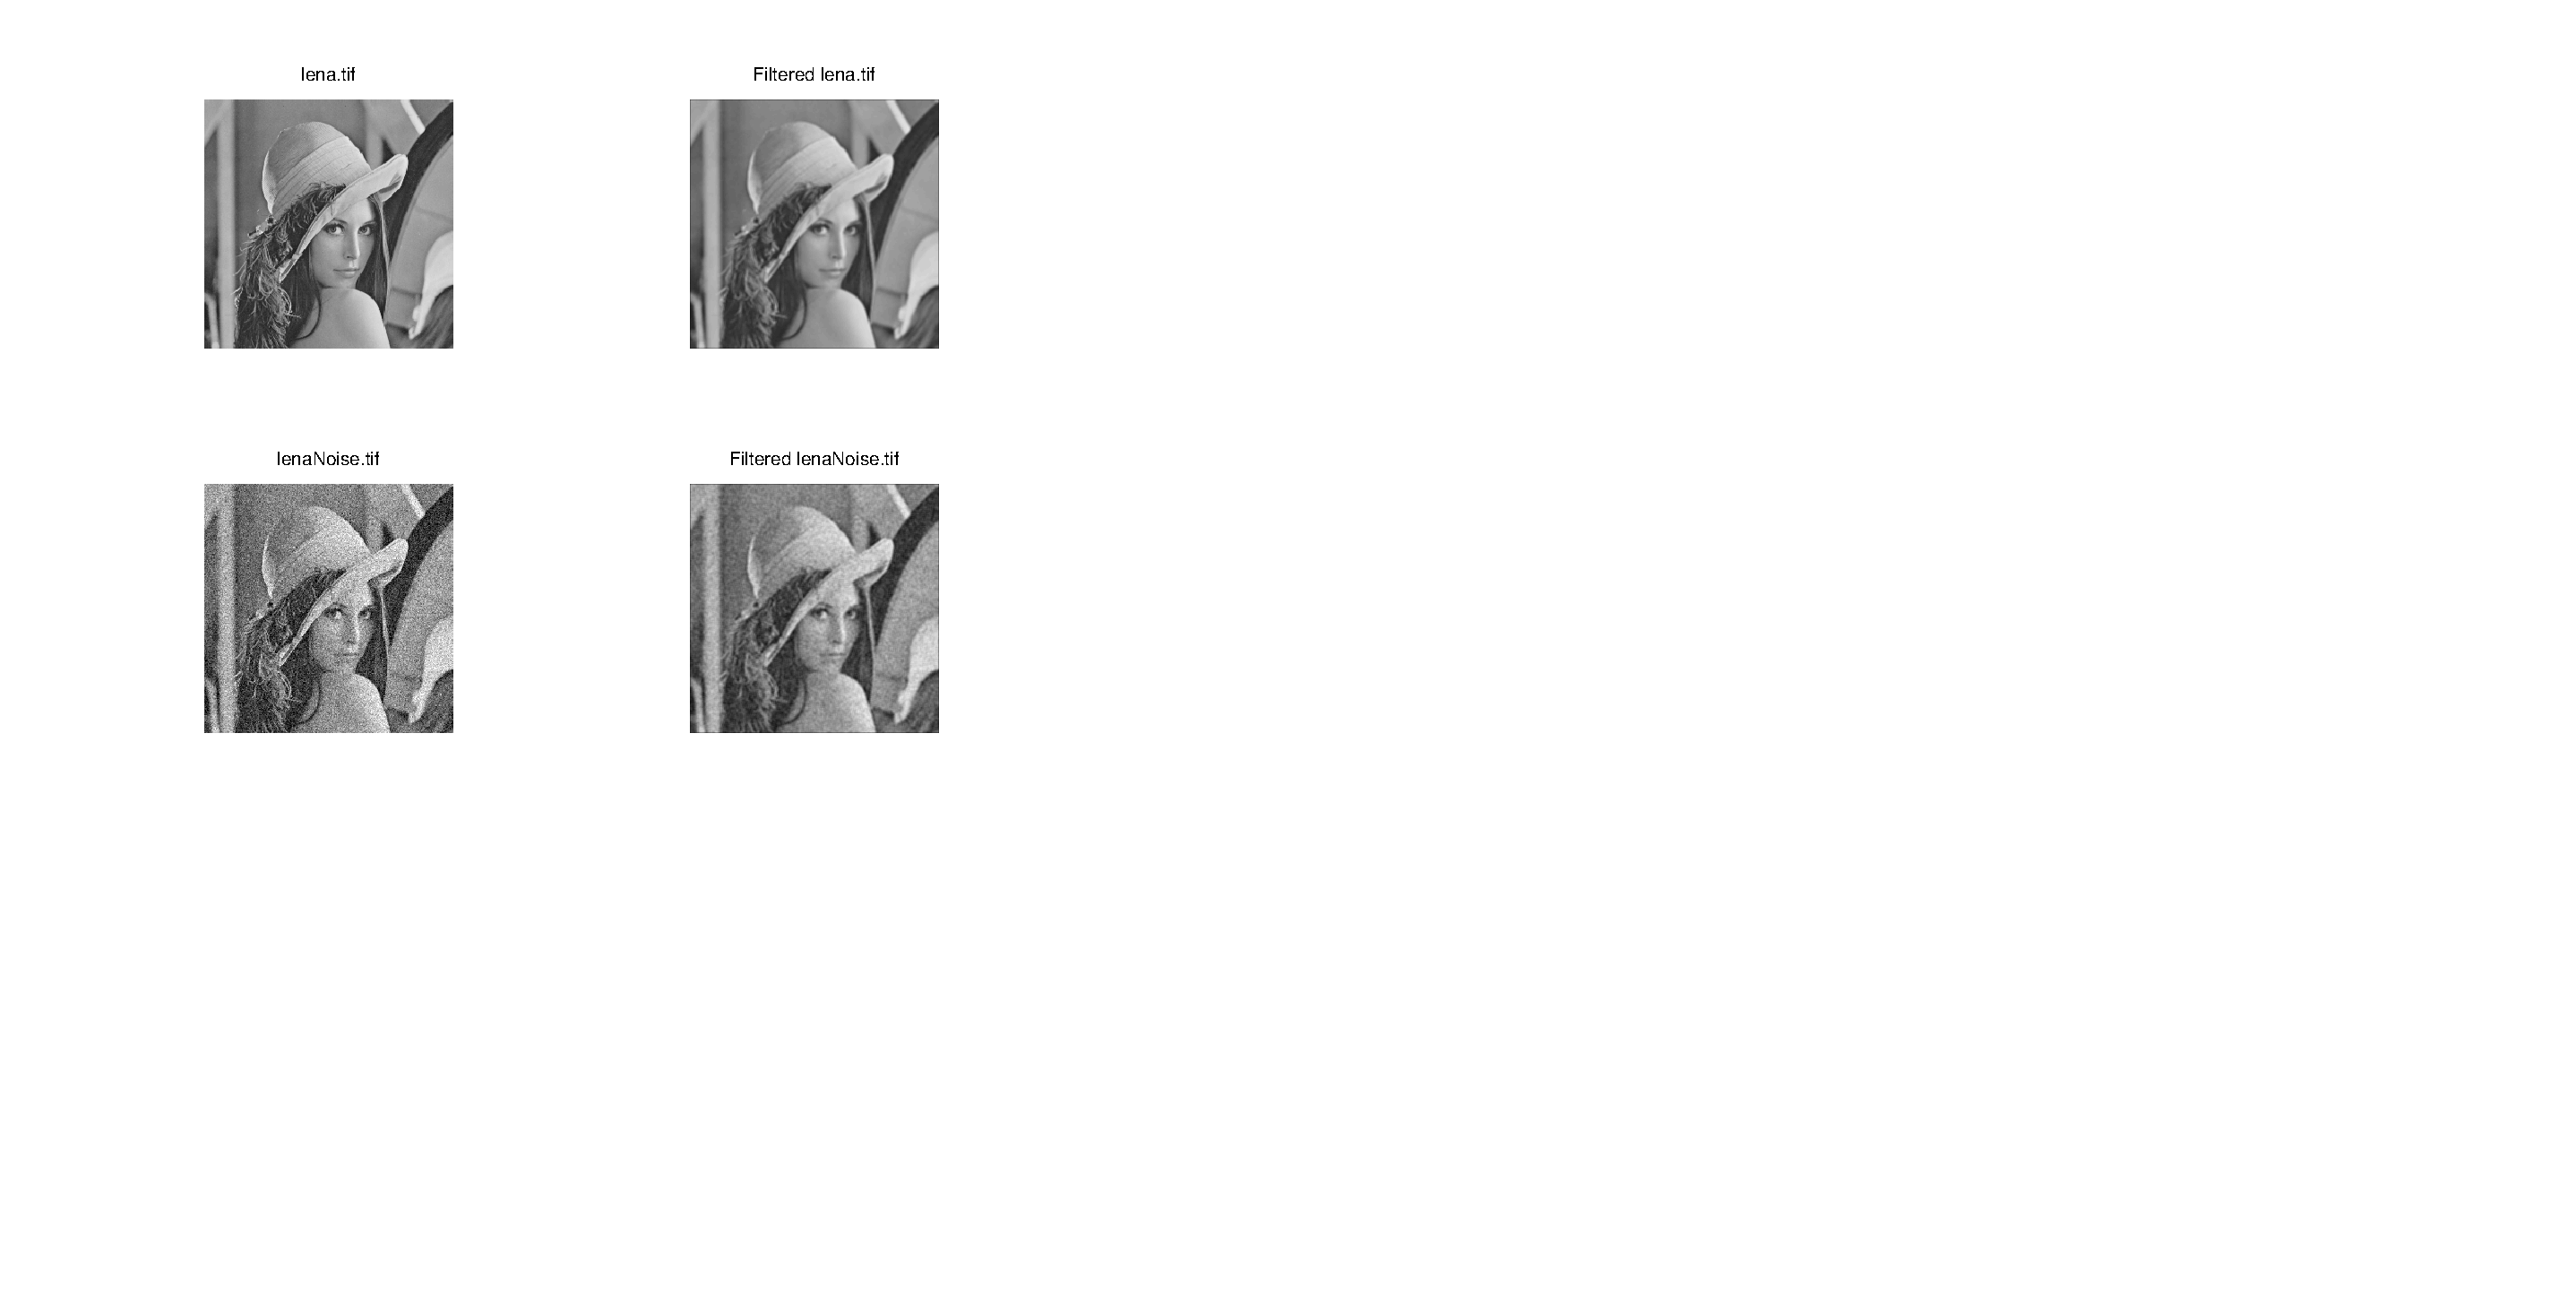
\includegraphics[trim = {0 9cm 27cm 0}, clip,width=\textwidth]{BoxFilter}
                \caption{Original and filtered images}
            \end{figure} 
    \end{enumerate}
\end{document}
